\documentclass[11pt]{article}

\usepackage{amsmath}
\usepackage{amsthm}
\usepackage{amsfonts}
\usepackage{hyperref}	
\usepackage{xcolor}	
\usepackage{graphicx}

\setlength{\textwidth}     {16.0cm}
\setlength{\textheight}    {21.0cm}
\setlength{\evensidemargin}{ 0.0cm}
\setlength{\oddsidemargin} { 0.0cm}
\setlength{\topmargin}     {-0.5cm}
\setlength{\baselineskip}  { 0.7cm}

\newcommand{\xkjtrial}{x^{k,j}_{\mathrm{trial}}}
\newcommand{\minimize}{\mathop{\text{Minimize}}}
\newcommand{\flow}{f_{\mathrm{low}}}

\newtheorem{theorem}{Theorem}[section]
\newtheorem{corollary}[theorem]{Corollary}
\newtheorem{lemma}[theorem]{Lemma}
\newtheorem{definition}[theorem]{Definition}
\newtheorem{assumption}{Assumption}
\renewcommand\theassumption{A\arabic{assumption}}

\newcounter{alg}[section]
\renewcommand{\thealg}{\thesection.\arabic{alg}}

% Show line numbers
\usepackage[mathlines]{lineno}
\renewcommand\linenumberfont{\normalfont\small\color{gray}}
% \linenumbers



\begin{document}

\title{A regularized Newton-type method for box-constrained order-value optimization}

\author{
    G. Q. Álvarez\thanks{Mathematics Program, Faculty of Basic Sciences, University of the Atlantic, Puerto Colombia, Atlántico, Colombia. e-mail: gdquintero@uniatlantico.edu.co}
    \and 
    C. A. Araujo\thanks{Mathematics Program, Faculty of Basic Sciences, University of the Atlantic, Puerto Colombia, Atlántico, Colombia. e-mail: carlosaraujo@uniatlantico.edu.co}
    \and
    M. A. C. Candezano\thanks{Mathematics Program, Faculty of Basic Sciences, University of the Atlantic, Puerto Colombia, Atlántico, Colombia. e-mail: miguelcaro@uniatlantico.edu.co}
}

% \date{June 18, 2025\footnote{Revision made on \today.}}
\date{\today}
\maketitle

\begin{abstract}
The order-value function of order $p$ returns, at each point, the $p$th
smallest value among a finite family $f_1,\dots,f_m$; minimizing it is a
flexible tool for robust estimation, in which a prescribed number of outlying
observations are discarded. We propose a regularized method for minimizing it
subject to box constraints. At each iteration the method minimizes a strongly
convex model combining a piecewise-linear term built from the active gradients,
a curvature term in which each active component carries its own symmetric
positive semidefinite matrix of norm at most $M$, and a quadratic
regularization. The curvature matrices are otherwise arbitrary, so quasi-Newton
updates, Gauss--Newton matrices and modified exact Hessians are all admissible,
and the first-order method is recovered when they vanish. Building on the
approximate optimality condition of the first-order method, we prove that the
method is well defined and attains worst-case iteration- and
evaluation-complexity bounds of the same order, the curvature entering only the
constants. Numerically, the curvature lowers the cost on a model nonlinear in
the parameters once outliers are discarded, and is neutral on a model affine in
them.

\medskip
\noindent
\textbf{Keywords:} Order-value optimization, regularized models,
Newton-type methods, complexity, algorithms, applications.

\medskip
\noindent
\textbf{Mathematics Subject Classification:} 90C30, 65K05, 49M37, 90C60, 68Q25.
\end{abstract}

\section{Introduction} \label{sec:intro}

Many optimization problems involve objective functions that are obtained not
by aggregating a collection of simpler functions, but by selecting one of them
according to its rank. The prototypical example is the order-value function of
order $p$, introduced in \cite{dunder1,dunder2}: given $m$ functions
$f_1,\dots,f_m$, its value at a point $x$ is the $p$th smallest among
$f_1(x),\dots,f_m(x)$. Functions of this kind belong to the broader class of
generalized order-value functions---those whose value at $x$ is governed by
order relations among the elements of a set $\{f_i(x)\}_{i\in I}$---a class
systematized in \cite{mtop}. Since the index that attains the $p$th position
may switch abruptly as $x$ moves, the order-value function is generally
nonsmooth even when each $f_i$ is continuously differentiable.

The extreme choices $p=1$ and $p=m$ recover the minimum and the maximum of
$\{f_i(x)\}$, respectively, so the order-value function interpolates between
these two classical aggregates; the intermediate cases are the ones of
practical interest. When $x$ encodes portfolio positions and $f_i(x)$ is the
loss incurred under scenario $i$, the order-value function coincides with the
discrete value-at-risk (VaR) measure, a standard risk measure in financial
risk management \cite{jorion}. When $f_i(x)$ measures the misfit of a
parametric model to the $i$th observation, minimizing the $p$th order-value
function fits the parameters while discarding the $m-p$ worst-fitted
observations. This makes order-value optimization a natural tool for robust
estimation, where one seeks to remain insensitive to a minority of grossly
corrupted data, or outliers.

The order-value optimization (OVO) problem was first formulated in
\cite{dunder1}, where a steepest-descent-type method was proposed and shown to
converge to points satisfying a weak optimality condition. Sharper optimality
conditions and a reformulation as a nonlinear program with equilibrium
constraints were subsequently developed in \cite{dunder2}. A quasi-Newton
method generalizing the Cauchy scheme of \cite{dunder1}---approximating the
active components by convex quadratics and proving global and local
convergence---was introduced in \cite{yano1}, and a global optimization
strategy combining multistart with a tunneling technique was proposed in
\cite{salva}. A closely related variant, in which the sum of the $p$ smallest
values is minimized---low order-value optimization (LOVO)---was developed with
applications to robust estimation and data analysis in \cite{yano2}. On the
computational-complexity side, \cite{jiang} established that minimizing the
order-value function over a polytope is NP-hard in the strong sense.

The systematic study of worst-case complexity in continuous optimization
originates in the cubic-regularization analysis of \cite{nesterov}, and
complexity guarantees have since been obtained for a broad range of problems
(see, e.g., \cite{bgmst2,bgmst1} and the monograph \cite{cogtbook}). Within
this line, \cite{alvarezovo} recently proposed a first-order method for
box-constrained OVO that minimizes, at each iteration, a quadratically
regularized piecewise-linear model of $f$, and established iteration- and
evaluation-complexity bounds for reaching an approximate optimality condition.

In the present work we generalize the approach of \cite{alvarezovo} by
enriching the regularized model with second-order information. At each
iteration our method minimizes a model built from the same piecewise-linear
convex term, a curvature term in which each active component $f_i$ carries its
own symmetric positive semidefinite matrix $B_i$ of norm at most $M$, and a
Tikhonov-type quadratic regularization. Beyond these two requirements the
matrices $B_i$ are arbitrary: a quasi-Newton update such as BFGS or SR1, a
Gauss--Newton matrix, or an exact component Hessian shifted to positive
definiteness are all admissible, and the analysis is indifferent to which is
used. The regularization renders the model strongly convex, so that each
subproblem has a unique minimizer. Setting $B_i=0$ recovers the
first-order method of \cite{alvarezovo} exactly, so the proposed method is a
strict generalization of it. Curvature had already been incorporated into OVO
by the quasi-Newton method of \cite{yano1}, which approximates the active
components by convex quadratics with positive semidefinite quasi-Newton
Hessians and establishes global convergence together with local superlinear
and quadratic rates; that method, however, controls the step through a
trust-region bound combined with a line search, and its guarantees are
asymptotic. Here the curvature is instead embedded in the adaptively
regularized model of \cite{alvarezovo}: the Tikhonov term renders each
subproblem strongly convex with a unique minimizer, and the analysis yields
non-asymptotic worst-case iteration- and evaluation-complexity bounds rather
than asymptotic convergence rates. Building on the approximate optimality
condition of \cite{alvarezovo} for
the box-constrained problem, we prove that the method is well defined and
attains worst-case iteration- and evaluation-complexity bounds of the
\emph{same order} as the first-order method (Theorem~\ref{teo:complexity}). Thus the incorporation of curvature does not degrade
the theoretical guarantees; whether it also yields a practical advantage is a
separate question, which we examine empirically on parameter-estimation
problems in the presence of outliers.

The remainder of the paper is organized as follows. Section~\ref{sec:method}
defines the box-constrained order-value optimization problem and the proposed
regularized method. Section~\ref{sec:complexity} introduces an appropriate
optimality condition and establishes the well-definiteness, convergence, and
complexity of the method. Section~\ref{sec:numerical} reports illustrative
numerical experiments on parameter estimation in the presence of outliers.
Final remarks are given in Section~\ref{sec:final}.

\medskip
\noindent\textit{Notation.} The symbol $\|\cdot\|$ denotes the Euclidean norm.
For $i=1,\dots,n$, $e_i\in\mathbb{R}^{n}$ denotes the $i$th column of the
identity matrix.

\section{A regularized Newton-type method} \label{sec:method}

Let $f_i : \mathbb{R}^n \to \mathbb{R}$, $i = 1, \ldots, m$, be given and let
$p \in \{1, \ldots, m\}$ be fixed. The \textit{order-value function of order
$p$} is the mapping $f : \mathbb{R}^n \to \mathbb{R}$ defined by
\begin{equation}
    f(x) = f_{i_p(x)}(x), \label{ovo-function}
\end{equation}
where $\{i_1(x), \ldots, i_m(x)\}$ is a permutation of $\{1, \ldots, m\}$ such
that
\begin{equation}
    f_{i_1(x)}(x) \leq f_{i_2(x)}(x) \leq \cdots \leq f_{i_m(x)}(x);
    \label{fi-sort}
\end{equation}
that is, $f(x)$ is the $p$th smallest value among $f_1(x), \ldots, f_m(x)$.
The boundary cases $p = 1$ and $p = m$ recover, respectively, the minimum and
the maximum of $\{f_1(x), \ldots, f_m(x)\}$.

If $f_1, \ldots, f_m$ are continuous, then so is $f$. Differentiability,
however, is not inherited: $f$ may be nonsmooth at a point $x$ at which the
$p$th smallest value is attained by more than one index, i.e.\ whenever there
exist $i \neq j$ with $f_i(x) = f_j(x) = f(x)$, since the active index $i_p(x)$
may then change as $x$ varies.

We address the box-constrained order-value optimization problem
\begin{equation}
    \minimize_{x \in \Omega} f(x), \label{ovo-problem}
\end{equation}
where $\Omega := \{x \in \mathbb{R}^n \mid \ell \leq x \leq u\}$ with
$\ell, u \in \mathbb{R}^n$ and $\ell_i < u_i$ for $i = 1, \ldots, n$. Box
constraints arise naturally in parameter estimation, where the unknowns are
confined to physically or statistically meaningful bounds.

For $\delta > 0$ and $x \in \Omega$, define the \textit{active index set}
\begin{equation}
    I_\delta(x) := \{i \in \{1, \ldots, m\} \mid
    f(x) - \delta \leq f_i(x) \leq f(x) + \delta\}, \label{idelta}
\end{equation}
the set of indices whose values lie within a band of half-width $\delta$ around
$f(x)$. As $\delta \to 0$, $I_\delta(x)$ shrinks to the set of indices that
attain the order-value,
\begin{equation*}
    I_0(x) := \{i \in \{1, \ldots, m\} \mid f_i(x) = f(x)\}.
\end{equation*}

The method builds, around a reference point $\bar{x} \in \Omega$, a local model
of $f$ that combines the first-order information of the active components with
curvature. Each component carries its own curvature matrix: given $M > 0$, we
call
\begin{equation*}
    \mathcal{B} = \{ B_i \}_{i=1}^{m}, \qquad
    B_i \in \mathbb{R}^{n \times n} \text{ symmetric},\ B_i \succeq 0,\
    \|B_i\| \leq M,
\end{equation*}
an \textit{admissible curvature family}; only those $B_i$ with
$i \in I_\delta(\bar{x})$ enter the model below. For given $\bar{x} \in \Omega$,
an admissible $\mathcal{B}$, $\delta \geq 0$, and $\sigma > 0$, the regularized
model is
\begin{equation}
    \Psi(x; \bar{x}, \mathcal{B}, \delta, \sigma) =
    \max_{i \in I_\delta(\bar{x})}
    \left\lbrace \nabla f_i(\bar{x})^T(x - \bar{x})
    + \frac{1}{2} \left[ (x - \bar{x})^T B_i (x - \bar{x})
    + \sigma \|x - \bar{x}\|^2 \right]\right\rbrace. \label{model}
\end{equation}
The first term is the piecewise-linear convex function that captures the
worst-case first-order behavior of $f$ over the active components; the bracket
adds the curvature $(x - \bar{x})^T B_i (x - \bar{x})$ of the $i$th component
and a Tikhonov regularization $\sigma \|x - \bar{x}\|^2$. Each component of the
maximum is a convex quadratic, so $\Psi$ is convex; since $\sigma > 0$ it is in
fact strongly convex even when the $B_i$ are only positive semidefinite, and the
subproblem \eqref{ovo-subpro} has a unique minimizer. Taking $B_i = 0$ for all
$i$ reduces the model to the first-order regularized model of
\cite{alvarezovo}, which the present method thus generalizes; taking a single
matrix $B_i \equiv B$ common to all active components is the intermediate case
in which one curvature matrix is shared.

\medskip
\noindent\refstepcounter{alg}\label{alg:main}\textbf{Algorithm~\thealg.} Let $\delta > 0$,
$\sigma_{\min} > 0$, $M > 0$, $\alpha \in (0,1)$, $\gamma > 1$, and
$x^0 \in \Omega$ be given. Initialize $k \leftarrow 0$.
\begin{description}
\item[Step~1.] Initialize $j \leftarrow 0$ and $\sigma_{k,j} = \sigma_{\min}$.
\item[Step~2.] Choose an admissible curvature family
$\mathcal{B}_{k,j} = \{B_{k,j,i}\}_{i=1}^{m}$ and compute
$\xkjtrial$ as the global minimizer of
    \begin{equation} \label{ovo-subpro}
    \minimize_{x \in \Omega}\, \Psi(x; x^k, \mathcal{B}_{k,j}, \delta, \sigma_{k,j}).
    \end{equation}
\item[Step~3.] If
    \begin{equation} \label{ovo-armijo}
    f(\xkjtrial) \leq f(x^k) - \alpha \|\xkjtrial - x^k\|^2
    \end{equation}
does not hold, set $\sigma_{k,j+1} = \gamma \sigma_{k,j}$,
$j \leftarrow j + 1$, and go to Step~2.
\item[Step~4.] Set $x^{k+1} = \xkjtrial$, $\sigma_k = \sigma_{k,j}$,
$j_k = j$, $k \leftarrow k+1$, and go to Step~1.
\end{description}

The bound $\|B_{k,j,i}\| \leq M$ keeps the curvature from dominating the model.
Positive semidefiniteness and that bound are the \emph{only} requirements: the
freedom in choosing the $B_{k,j,i}$ lets the method accommodate standard
quasi-Newton updates such as BFGS or SR1, Gauss--Newton matrices, and exact
component Hessians shifted to positive definiteness, while the choice
$B_{k,j,i} = 0$ for all $k, j, i$ recovers the first-order method of
\cite{alvarezovo}. The analysis below is indifferent to which of these is used.

The requirements on $\xkjtrial$ are mild. The theory only needs $\xkjtrial$ to
be a stationary point of \eqref{ovo-subpro} with
$\Psi(\xkjtrial; x^k, \mathcal{B}_{k,j}, \delta, \sigma_{k,j}) \leq 0$; since
$\Psi(x^k; x^k, \mathcal{B}_{k,j}, \delta, \sigma_{k,j}) = 0$, any descent method started
at $x^k$ produces such iterates. Moreover, \eqref{ovo-subpro} minimizes a
strongly convex function over the compact convex set $\Omega$, so it has a
unique global minimizer and every stationary point is global; the
global-minimizer requirement of Step~2 is therefore met by any such descent
method, and standard convex solvers apply directly.

\section{Optimality condition and complexity} \label{sec:complexity}

\begin{assumption} \label{a1}
The functions $f_1, \ldots, f_m$ belong to $\mathcal{C}^1(\Omega)$; that is,
they are continuously differentiable on $\Omega$.
\end{assumption}

We first show that a local minimizer of \eqref{ovo-problem} also minimizes the
model $\Psi$ built at the corresponding reference point. These results connect
the original nonsmooth problem with the convex subproblems solved at each
iteration and underlie the optimality condition introduced below. Throughout,
$\mathcal{O}$ denotes the admissible curvature family with $B_i = 0$ for all
$i$.

\begin{theorem} \label{teo:conv1}
Suppose that Assumption~\ref{a1} holds. If $x^*$ is a local minimizer of
\eqref{ovo-problem}, then it is also a local minimizer of
$\minimize_{x \in \Omega}\, \Psi(x; x^*, \mathcal{O}, 0, 0)$.
\end{theorem}

\begin{proof}
Suppose not. Then there is $y^* \in \Omega$ with
$\Psi(y^*; x^*, \mathcal{O}, 0, 0) < \Psi(x^*; x^*, \mathcal{O}, 0, 0) = 0$, i.e.\
$\nabla f_i(x^*)^T(y^* - x^*) < 0$ for all $i \in I_0(x^*)$. By
Assumption~\ref{a1}, for each such $i$,
\[
\lim_{t \to 0^+} \frac{f_i(x^* + t(y^* - x^*)) - f_i(x^*)}{t}
= \nabla f_i(x^*)^T(y^* - x^*) < 0,
\]
so there is $\bar{t}_i > 0$ with $f_i(x^* + t(y^* - x^*)) < f_i(x^*) = f(x^*)$
for $t \in (0, \bar{t}_i]$. With $\bar{t} = \min_{i \in I_0(x^*)} \bar{t}_i$,
\begin{equation} \label{bajaste}
f_i(x^* + t(y^* - x^*)) < f(x^*) \quad
\text{for all } i \in I_0(x^*),\ t \in (0, \bar{t}].
\end{equation}
For $j \notin I_0(x^*)$, continuity of $f_1, \ldots, f_m$ gives, for $t$ small,
\begin{align}
f_i(x^* + t(y^* - x^*)) &< f_j(x^* + t(y^* - x^*))
&&\text{if } i \in I_0(x^*),\ f(x^*) < f_j(x^*), \label{arriba}\\
f_i(x^* + t(y^* - x^*)) &> f_j(x^* + t(y^* - x^*))
&&\text{if } i \in I_0(x^*),\ f(x^*) > f_j(x^*). \label{abajo}
\end{align}
Hence the ranking positions of the active indices $I_0(x^*)$ within
$\{f_i(x^* + t(y^* - x^*))\}_{i=1}^m$ are preserved for $t$ small, so the $p$th
position is still occupied by some $i \in I_0(x^*)$ and
$f(x^* + t(y^* - x^*)) = f_i(x^* + t(y^* - x^*))$. With \eqref{bajaste},
$f(x^* + t(y^* - x^*)) < f(x^*)$ for $t$ small. Since $\Omega$ is convex,
$x^* + t(y^* - x^*) \in \Omega$, contradicting the local minimality of $x^*$.
\end{proof}

\begin{theorem} \label{teo:conv2}
Suppose that Assumption~\ref{a1} holds and let $\mathcal{B}$ be an admissible
curvature family and $\sigma \geq 0$. If $x^*$ is a local minimizer of
\eqref{ovo-problem}, then it is also a local minimizer of
\[
\minimize_{x \in \Omega}\, \Psi(x; x^*, \mathcal{B}, 0, \sigma).
\]
\end{theorem}

\begin{proof}
Suppose not: there is $y^* \in \Omega$ with
$\Psi(y^*; x^*, \mathcal{B}, 0, \sigma) < 0$. Since the model is a maximum over
$i \in I_0(x^*)$, every one of its components is negative at $y^*$:
\[
\nabla f_i(x^*)^T(y^* - x^*)
+ \tfrac{1}{2} \big[ (y^* - x^*)^T B_i (y^* - x^*) + \sigma \|y^* - x^*\|^2 \big]
< 0 \qquad \text{for all } i \in I_0(x^*).
\]
Since $B_i \succeq 0$ and $\sigma \geq 0$, each bracket is nonnegative, so
$\nabla f_i(x^*)^T(y^* - x^*) < 0$ for every $i \in I_0(x^*)$, and therefore
$\max_{i \in I_0(x^*)} \{ \nabla f_i(x^*)^T(y^* - x^*) \} < 0$, that is,
$\Psi(y^*; x^*, \mathcal{O}, 0, 0) < 0$. This contradicts
Theorem~\ref{teo:conv1}.
\end{proof}

\begin{theorem} \label{teo:conv3}
Suppose that Assumption~\ref{a1} holds and let $\mathcal{B}$ be an admissible
curvature family and $\sigma, \delta \geq 0$. If $x^*$ is a local minimizer of
\eqref{ovo-problem}, then it is also a local minimizer of
$\minimize_{x \in \Omega}\, \Psi(x; x^*, \mathcal{B}, \delta, \sigma)$.
\end{theorem}

\begin{proof}
Suppose not: there is $y^* \in \Omega$ with
$\Psi(y^*; x^*, \mathcal{B}, \delta, \sigma) < 0$. Both models are maxima of the
same family of functions, taken over $I_0(x^*)$ and over $I_\delta(x^*)$
respectively; since $I_0(x^*) \subseteq I_\delta(x^*)$, the maximum over the
smaller index set is no larger, so
\[
\Psi(y^*; x^*, \mathcal{B}, 0, \sigma)
\leq \Psi(y^*; x^*, \mathcal{B}, \delta, \sigma) < 0,
\]
contradicting Theorem~\ref{teo:conv2}.
\end{proof}

Throughout, $\Sigma_q := \{ \lambda \in \mathbb{R}^q \mid
\sum_{j=1}^q \lambda_j = 1,\ \lambda_j \geq 0 \}$ denotes the unit simplex.
Following \cite{alvarezovo}, the next consequence of Theorem~\ref{teo:conv3}
provides a first-order necessary condition for \eqref{ovo-problem} and
motivates the stopping criterion below.

\begin{corollary} \label{cor:exact}
Suppose that Assumption~\ref{a1} holds and let $\delta \geq 0$. If $x^*$ is a
local minimizer of \eqref{ovo-problem}, then there exist
$\mu \in \Sigma_{|I_\delta(x^*)|}$ and $\nu^\ell, \nu^u \in \mathbb{R}^n_+$ such
that $(\ell_i - x^*_i)\nu^\ell_i = (x^*_i - u_i)\nu^u_i = 0$ for
$i = 1, \ldots, n$ and
\begin{equation} \label{exact-opt}
\sum_{i \in I_\delta(x^*)} \mu_i \nabla f_i(x^*)
+ \sum_{i=1}^n (\nu^u_i - \nu^\ell_i) e_i = 0.
\end{equation}
\end{corollary}

\begin{proof}
By Theorem~\ref{teo:conv3} with $B_i = 0$ for all $i$ and $\sigma = 0$, the
point $x^*$ minimizes
$x \mapsto \max_{i \in I_\delta(x^*)} \{ \nabla f_i(x^*)^T(x - x^*) \}$ over
$\Omega$. Applying the KKT conditions for the minimization of a maximum of
differentiable functions over a box (Lemma~3.1 of \cite{alvarezovo}) yields
multipliers $\mu \in \Sigma_{|I_\delta(x^*)|}$ and
$\nu^\ell, \nu^u \in \mathbb{R}^n_+$ with the stated complementarity and
\eqref{exact-opt}.
\end{proof}

\begin{definition} \label{def:optcond}
Given $\epsilon > 0$ and $\delta > 0$, we say that $x \in \Omega$ satisfies the
\textit{approximate optimality condition} $C_{\delta,\epsilon}$ if there exist
$\mu \in \Sigma_{|I_\delta(x)|}$ and $\nu^\ell, \nu^u \in \mathbb{R}^n_+$ such
that $(\ell_i - x_i)\nu^\ell_i = (x_i - u_i)\nu^u_i = 0$ for $i = 1, \ldots, n$
and
\begin{equation} \label{miaprox-box}
\left\| \sum_{i \in I_\delta(x)} \mu_i \nabla f_i(x)
+ \sum_{i=1}^{n} (\nu^u_i - \nu^\ell_i) e_i \right\| \leq \epsilon.
\end{equation}
\end{definition}

Condition $C_{\delta,\epsilon}$ requires the gradient combination of the active
components, corrected by the box multipliers, to be small in norm. For
$\epsilon = 0$ it reduces to the exact condition \eqref{exact-opt} of
Corollary~\ref{cor:exact}. This condition was introduced in \cite{alvarezovo}
for the first-order method; we adopt it unchanged, since it involves only the
active gradients and the box multipliers and is therefore insensitive to the
curvature. It serves as the stopping criterion for
Algorithm~\ref{alg:main}.

\begin{corollary} \label{cor:step}
Suppose that Assumption~\ref{a1} holds. Then, for every $k$ and
$j = 0, \ldots, j_k$, there exist $\mu \in \Sigma_{|I_\delta(x^k)|}$ and
$\nu^\ell, \nu^u \in \mathbb{R}^n_+$ such that
$(\ell_i - [\xkjtrial]_i)\nu^\ell_i = ([\xkjtrial]_i - u_i)\nu^u_i = 0$ for
$i = 1, \ldots, n$ and
\begin{equation} \label{eqcoro1}
\xkjtrial - x^k = \big( \bar{B}_{k,j} + \sigma_{k,j} I \big)^{-1}
\left[ \sum_{i=1}^{n} (\nu^\ell_i - \nu^u_i) e_i
- \sum_{i \in I_\delta(x^k)} \mu_i \nabla f_i(x^k) \right],
\end{equation}
where
\begin{equation} \label{bbar}
\bar{B}_{k,j} := \sum_{i \in I_\delta(x^k)} \mu_i B_{k,j,i}
\end{equation}
is symmetric, positive semidefinite, and satisfies
$\|\bar{B}_{k,j}\| \leq M$.
\end{corollary}

\begin{proof}
Subproblem \eqref{ovo-subpro} minimizes the strongly convex function
$\Psi(\cdot\,; x^k, \mathcal{B}_{k,j}, \delta, \sigma_{k,j})$ over the box
$\Omega$. By
the KKT conditions for a maximum of differentiable functions over a box
(Lemma~3.1 of \cite{alvarezovo}), there exist $\mu \in \Sigma_{|I_\delta(x^k)|}$ and
$\nu^\ell, \nu^u \in \mathbb{R}^n_+$ with the stated complementarity such that
\[
\sum_{i \in I_\delta(x^k)} \mu_i
\big[ \nabla f_i(x^k) + (B_{k,j,i} + \sigma_{k,j} I)(\xkjtrial - x^k) \big]
+ \sum_{i=1}^n (\nu^u_i - \nu^\ell_i) e_i = 0,
\]
where $\nabla f_i(x^k) + (B_{k,j,i} + \sigma_{k,j} I)(\xkjtrial - x^k)$ is the
gradient at $\xkjtrial$ of the $i$th component of $\Psi$. Since
$\sum_i \mu_i = 1$, the terms involving $\sigma_{k,j}$ collect into
$\sigma_{k,j}(\xkjtrial - x^k)$ and those involving the curvature into
$\bar{B}_{k,j}(\xkjtrial - x^k)$ with $\bar{B}_{k,j}$ given by \eqref{bbar}.
Being a convex combination of symmetric positive semidefinite matrices,
$\bar{B}_{k,j}$ is itself symmetric and positive semidefinite, and
$\|\bar{B}_{k,j}\| \leq \sum_{i \in I_\delta(x^k)} \mu_i \|B_{k,j,i}\| \leq M$.
As $\sigma_{k,j} > 0$ and $\bar{B}_{k,j} \succeq 0$, the matrix
$\bar{B}_{k,j} + \sigma_{k,j} I$ is positive definite, and solving for
$\xkjtrial - x^k$ gives \eqref{eqcoro1}.
\end{proof}

\begin{assumption} \label{a2}
For all $k$ and $j = 0, \ldots, j_k$, the multipliers $\nu^\ell, \nu^u$ of
Corollary~\ref{cor:step} satisfy
$\max_{i = 1, \ldots, n} |\nu^\ell_i - \nu^u_i| \leq c_\nu$ for some constant
$c_\nu > 0$ independent of $k$ and $j$.
\end{assumption}

The Mangasarian--Fromovitz constraint qualification guarantees that, for each
$(k,j)$, these multipliers are bounded \cite{gauvin}; Assumption~\ref{a2}
strengthens this to a single bound uniform in $k$ and $j$, which is natural
since $\Omega$ is compact and the active gradients are bounded under
Assumption~\ref{a1}.

\begin{assumption} \label{a3}
There is a constant $c_\nabla > 0$ such that $\|\nabla f_i(x)\| \leq c_\nabla$
for all $i = 1, \ldots, m$ and all $x \in \Omega$.
\end{assumption}

Assumption~\ref{a3} holds automatically under Assumption~\ref{a1}, since
$\Omega$ is bounded. Combining Corollary~\ref{cor:step} with
Assumptions~\ref{a2} and~\ref{a3} bounds the step. Since
$\bar{B}_{k,j} \succeq 0$, the eigenvalues of
$\bar{B}_{k,j} + \sigma_{k,j} I$ are at least $\sigma_{k,j}$, so
$\|(\bar{B}_{k,j} + \sigma_{k,j} I)^{-1}\| \leq 1/\sigma_{k,j}$, and
\eqref{eqcoro1} gives
\[
\|\xkjtrial - x^k\| \leq \frac{1}{\sigma_{k,j}}
\left( \sum_{i=1}^n |\nu^\ell_i - \nu^u_i|
+ \sum_{i \in I_\delta(x^k)} \mu_i \|\nabla f_i(x^k)\| \right)
\leq \frac{n\,c_\nu + c_\nabla}{\sigma_{k,j}},
\]
where the last inequality uses Assumptions~\ref{a2}, \ref{a3} and
$\mu \in \Sigma_{|I_\delta(x^k)|}$. Thus
\begin{equation} \label{ccotasub}
\|\xkjtrial - x^k\| \leq \frac{c_x}{\sigma_{k,j}}, \qquad
c_x := n\,c_\nu + c_\nabla.
\end{equation}
The step shrinks as $\sigma_{k,j}$ grows, which is the mechanism driving the
acceptance of \eqref{ovo-armijo}.

\begin{assumption} \label{a4}
There is $L > 0$ such that $\|\nabla f_i(y) - \nabla f_i(x)\| \leq L \|y - x\|$
for all $i = 1, \ldots, m$ and $x, y \in \Omega$.
\end{assumption}

Assumption~\ref{a4} is the standard gradient-Lipschitz condition. It implies,
for all $i$ and $x, y \in \Omega$,
\begin{equation} \label{taylor}
f_i(y) \leq f_i(x) + \nabla f_i(x)^T(y - x) + \tfrac{L}{2}\|y - x\|^2,
\end{equation}
as well as the two-sided bound
$|f_i(y) - f_i(x) - \nabla f_i(x)^T(y - x)| \leq \tfrac{L}{2}\|y - x\|^2$. These
make $\Psi$ an upper model of $f$ once $\sigma_{k,j}$ is large relative to $L$,
which yields finite termination of the inner loop. 

\begin{lemma} \label{lem1}
Let $a_1, \ldots, a_r, b_1, \ldots, b_r \in \mathbb{R}$ and $\beta > 0$ satisfy
$a_1 \leq \cdots \leq a_r$, $b_j \leq a_j - \beta$ for $j = 1, \ldots, r$, and
$b_{i_1} \leq \cdots \leq b_{i_r}$ for a permutation $\{i_1, \ldots, i_r\}$ of
$\{1, \ldots, r\}$. Then $b_{i_q} \leq a_q - \beta$ for $q = 1, \ldots, r$.
\end{lemma}

\begin{proof}
See Lemma~2.1 of \cite{dunder1}.
\end{proof}

The next result gives a threshold on $\sigma_{k,j}$ beyond which the trial point
is accepted at Step~3, so that the inner loop terminates after finitely many
increases of $\sigma_{k,j}$, independently of $k$. The threshold scales with
$\delta^{-1}$: a narrower active band demands stronger regularization.

\begin{theorem} \label{teo:suff-descent}
Suppose that Assumptions~\ref{a1}, \ref{a2}, \ref{a3}, and \ref{a4} hold. Then,
for all $k$ and $j = 0, \ldots, j_k$, if
\begin{equation} \label{este}
\sigma_{k,j} \geq \max\{ L + 2\alpha,\ 9c_x^2/(2\delta) \},
\end{equation}
then $\xkjtrial$ satisfies \eqref{ovo-armijo}.
\end{theorem}

\begin{proof}
Assume \eqref{este}; in particular $\sigma_{k,j} \geq L + 2\alpha$. By
\eqref{taylor}, for every $i \in \{1, \ldots, m\}$,
\begin{align*}
f_i(\xkjtrial)
&\leq f_i(x^k) + \nabla f_i(x^k)^T(\xkjtrial - x^k)
+ \tfrac{L}{2}\|\xkjtrial - x^k\|^2 \\
&\leq f_i(x^k) + \nabla f_i(x^k)^T(\xkjtrial - x^k)
+ \Big( \tfrac{\sigma_{k,j}}{2} - \alpha \Big) \|\xkjtrial - x^k\|^2 \\
&= f_i(x^k) + \nabla f_i(x^k)^T(\xkjtrial - x^k) \\
&\quad + \tfrac{1}{2} \big[ (\xkjtrial - x^k)^T B_{k,j,i} (\xkjtrial - x^k)
+ \sigma_{k,j}\|\xkjtrial - x^k\|^2 \big] \\
&\quad - \alpha \|\xkjtrial - x^k\|^2
- \tfrac{1}{2}(\xkjtrial - x^k)^T B_{k,j,i} (\xkjtrial - x^k).
\end{align*}
Since $B_{k,j,i} \succeq 0$, the last term is nonpositive and may be dropped. For
$i \in I_\delta(x^k)$, the minimizer property
$\Psi(\xkjtrial; x^k, \mathcal{B}_{k,j}, \delta, \sigma_{k,j}) \leq
\Psi(x^k; x^k, \mathcal{B}_{k,j}, \delta, \sigma_{k,j}) = 0$ gives, since the
model is a maximum over $I_\delta(x^k)$ and therefore bounds each of its
components,
\[
\nabla f_i(x^k)^T(\xkjtrial - x^k)
+ \tfrac{1}{2} \big[ (\xkjtrial - x^k)^T B_{k,j,i} (\xkjtrial - x^k)
+ \sigma_{k,j}\|\xkjtrial - x^k\|^2 \big] \leq 0,
\]
so that
\begin{equation} \label{cota-lem2}
f_i(\xkjtrial) \leq f_i(x^k) - \alpha \|\xkjtrial - x^k\|^2, \qquad
i \in I_\delta(x^k).
\end{equation}
On the other hand, by \eqref{ccotasub}, the Cauchy--Schwarz inequality, and the
two-sided consequence of Assumption~\ref{a4}, using
$\|\nabla f_i(x^k)\| \leq c_\nabla \leq c_x$ and \eqref{ccotasub},
$|f_i(\xkjtrial) - f_i(x^k)| \leq c_x^2/\sigma_{k,j}
+ L c_x^2/(2\sigma_{k,j}^2)$ for all $i$; using $L \leq \sigma_{k,j}$, this is
at most $3c_x^2/(2\sigma_{k,j})$, and \eqref{este} yields
\begin{equation} \label{teo7eq1}
|f_i(\xkjtrial) - f_i(x^k)| \leq \tfrac{\delta}{3}, \qquad i = 1, \ldots, m.
\end{equation}
Write $\beta := \alpha\|\xkjtrial - x^k\|^2$ and let
$B := \{ i \mid f_i(x^k) < f(x^k) - \delta \}$ be the set of indices lying
strictly below the band at $x^k$, with $b := |B|$. Order the band as
$I_\delta(x^k) = \{i_1, \ldots, i_r\}$ with
$f_{i_1}(x^k) \leq \cdots \leq f_{i_r}(x^k)$; since every index of $B$ has a
value smaller than every index of the band, and every index above the band has
a larger one, the $p$th smallest value at $x^k$ is attained at position $q$ of
the band, where $b + q = p$; that is, $i_p(x^k) = i_q$ and
$f_{i_q}(x^k) = f(x^k)$.

Consider now the $p$ indices of $B \cup \{i_1, \ldots, i_q\}$. For $i \in B$,
\eqref{teo7eq1} gives
$f_i(\xkjtrial) \leq f_i(x^k) + \delta/3 < f(x^k) - 2\delta/3$, which is at
most $f(x^k) - \beta$ provided $\beta \leq 2\delta/3$; and indeed
\eqref{ccotasub} gives
\[
\beta = \alpha \|\xkjtrial - x^k\|^2 \leq \frac{\alpha c_x^2}{\sigma_{k,j}^2}
= \frac{\alpha}{\sigma_{k,j}} \cdot \frac{c_x^2}{\sigma_{k,j}}
\leq \frac{1}{2} \cdot \frac{2\delta}{9} = \frac{\delta}{9},
\]
where $c_x^2/\sigma_{k,j} \leq 2\delta/9$ and $\alpha/\sigma_{k,j} \leq 1/2$
follow from the two bounds in \eqref{este}. For
$i \in \{i_1, \ldots, i_q\} \subseteq I_\delta(x^k)$, \eqref{cota-lem2} together
with $f_i(x^k) \leq f_{i_q}(x^k) = f(x^k)$ gives
$f_i(\xkjtrial) \leq f_i(x^k) - \beta \leq f(x^k) - \beta$. Hence at least $p$
of the values $f_1(\xkjtrial), \ldots, f_m(\xkjtrial)$ are bounded above by
$f(x^k) - \beta$, and therefore so is the $p$th smallest among them:
\[
f(\xkjtrial) \leq f(x^k) - \beta = f(x^k) - \alpha\|\xkjtrial - x^k\|^2,
\]
which is \eqref{ovo-armijo}.
\end{proof}

The inner loop thus terminates finitely at every outer iteration. The curvature
affects only the constants below ---through the bound $M$ on $\|B_{k,j,i}\|$--- and
not the $O(\delta^{-2}\epsilon^{-2})$ iteration order, which coincides with that
of the first-order method \cite{alvarezovo}.

\begin{theorem} \label{teo:complexity}
Suppose that Assumptions~\ref{a1}, \ref{a2}, \ref{a3}, and \ref{a4} hold and
that there is
$\flow \in \mathbb{R}$ with $f(x) \geq \flow$ for all $x \in \Omega$. Then
\begin{equation} \label{cota-sigma}
\sigma_k \leq \gamma \max\{ L + 2\alpha,\ 9c_x^2/(2\delta) \},
\end{equation}
and at most
\begin{equation} \label{cota-fcnt}
\big\lfloor 1 + \log_\gamma( \sigma_k / \sigma_{\min} ) \big\rfloor
\end{equation}
function evaluations are performed per outer iteration to obtain
\eqref{ovo-armijo}. Moreover, the number of outer iterations $k$ at which the
multipliers of Corollary~\ref{cor:step} associated with $x^{k+1}$ do not
certify $C_{\delta,\epsilon}$ is at most
\begin{equation} \label{cota-iter}
\left\lfloor \frac{\big( M + \gamma \max\{ L + 2\alpha,\ 9c_x^2/(2\delta) \}
\big)^2}{\alpha} \cdot \frac{f(x^0) - \flow}{\epsilon^2} \right\rfloor.
\end{equation}
\end{theorem}

\begin{proof}
Bounds \eqref{cota-sigma} and \eqref{cota-fcnt} follow from
Theorem~\ref{teo:suff-descent} and the rule
$\sigma_{k,j+1} = \gamma\sigma_{k,j}$: starting from
$\sigma_{k,0} = \sigma_{\min}$, at most
$\lfloor 1 + \log_\gamma(\sigma_k/\sigma_{\min}) \rfloor$ increases occur before
\eqref{este} holds, after which \eqref{ovo-armijo} is satisfied.

Let $K$ be the set of outer indices $k$ for which the multipliers
$\mu, \nu^\ell, \nu^u$ furnished by Corollary~\ref{cor:step} at the accepted
trial point $x^{k+1}$ satisfy
$\| \sum_{i \in I_\delta(x^k)} \mu_i \nabla f_i(x^k)
+ \sum_{i=1}^n (\nu^u_i - \nu^\ell_i) e_i \| > \epsilon$; these multipliers are
precisely the ones the algorithm inspects at the stopping test, and the
condition $C_{\delta,\epsilon}$ is declared satisfied when this quantity does
not exceed $\epsilon$. Fix $k \in K$ and write
$\bar{B}_k = \bar{B}_{k,j_k}$, the convex
combination \eqref{bbar} associated with the accepted trial point. By
Corollary~\ref{cor:step},
$(\bar{B}_k + \sigma_k I)(x^{k+1} - x^k)
= \sum_{i=1}^n (\nu^\ell_i - \nu^u_i) e_i
- \sum_{i \in I_\delta(x^k)} \mu_i \nabla f_i(x^k)$, hence
\[
\big\| (\bar{B}_k + \sigma_k I)(x^{k+1} - x^k) \big\|
= \Big\| \sum_{i \in I_\delta(x^k)} \mu_i \nabla f_i(x^k)
+ \sum_{i=1}^n (\nu^u_i - \nu^\ell_i) e_i \Big\| > \epsilon .
\]
Since $\|\bar{B}_k\| \leq M$ by Corollary~\ref{cor:step},
\[
\epsilon < \| (\bar{B}_k + \sigma_k I)(x^{k+1} - x^k) \|
\leq (M + \sigma_k) \|x^{k+1} - x^k\|,
\]
and with \eqref{cota-sigma},
$\|x^{k+1} - x^k\| > \epsilon / \big( M + \gamma\max\{L + 2\alpha, 9c_x^2/(2\delta)\} \big)$.
As $x^{k+1}$ satisfies \eqref{ovo-armijo},
\[
f(x^{k+1}) \leq f(x^k) - \alpha\|x^{k+1} - x^k\|^2
< f(x^k) - \frac{\alpha\epsilon^2}
{\big( M + \gamma\max\{L + 2\alpha, 9c_x^2/(2\delta)\} \big)^2}.
\]
Summing over $k \in K$ and using $f(x) \geq \flow$ gives
$f(x^0) - \flow > |K| \cdot \alpha\epsilon^2 /
\big( M + \gamma\max\{L + 2\alpha, 9c_x^2/(2\delta)\} \big)^2$, from which
\eqref{cota-iter} follows.
\end{proof}

\section{Numerical experiments} \label{sec:numerical}

We illustrate the method on parameter-estimation problems in which the data
contain an unknown number of outliers, following the OVO methodology of
\cite{alvarezovo}. Given a model $y(t,x)$ with parameters $x\in\Omega$ and data
$(t_i,y_i)$, $i=1,\dots,m$, we set
\[
f_i(x)=\tfrac12\big(y(t_i,x)-y_i\big)^2,\qquad i=1,\dots,m.
\]
For a prescribed number $o$ of outliers, solving \eqref{ovo-problem} with
$p=m-o$ fits the parameters to the $p$ best-explained observations while
discarding the $o$ worst. Since the true number of outliers is unknown, we
solve a sequence of OVO problems with increasing $o$; a sharp drop in $f(x^*)$
identifies the number of outliers present.

Our aim is to assess the effect of the curvature. We therefore compare two
instances of Algorithm~\ref{alg:main} that differ \emph{only} in the curvature
family: the first-order method ($B_{k,j,i}=0$ for all $i$, which coincides with
\cite{alvarezovo}) and a second-order variant, in which each active component
contributes its own matrix. For the least-squares functions above,
$\nabla f_i(x)=r_i(x)\nabla r_i(x)$ and
\[
\nabla^2 f_i(x)=\nabla r_i(x)\nabla r_i(x)^T + r_i(x)\nabla^2 r_i(x),
\qquad r_i(x)=y(t_i,x)-y_i .
\]
We take $B_{k,j,i}$ to be the exact component Hessian $\nabla^2 f_i(x^k)$,
made positive definite by the shift
\begin{equation} \label{shift}
B_{k,j,i} \leftarrow \nabla^2 f_i(x^k)
+ \max\big\{0,\ -\lambda_{\min}\big(\nabla^2 f_i(x^k)\big) + \tau \big\}\, I,
\qquad \tau = 10^{-8},
\end{equation}
and then rescaled by $M/\lambda_{\max}(B_{k,j,i})$ whenever
$\lambda_{\max}(B_{k,j,i}) > M$, so that the requirements $B_{k,j,i}\succeq0$
and $\|B_{k,j,i}\|\le M$ of Step~2 hold. The eigenvalues are computed with the
LAPACK routine \texttt{DSYEV}. For the model of Section~\ref{subsec:poly},
which is affine in the parameters, $\nabla^2 r_i=0$ and the component Hessian
reduces to the constant Gauss--Newton matrix $\nabla r_i\nabla r_i^T$, already
positive semidefinite, so the shift in \eqref{shift} is inactive up to $\tau$;
for the nonlinear model of Section~\ref{subsec:bard} the term
$r_i\nabla^2 r_i$ is present, the component Hessians are indefinite in general,
and the shift is genuinely active. Quasi-Newton updates such as BFGS or SR1 are
equally admissible in Step~2; we use exact Hessians here because $\nabla^2 r_i$
is available in closed form for both test problems, which isolates the effect
of the curvature itself from that of any approximation to it. Like $\delta$,
the value of $M$ is chosen by trial and error.

As in \cite{alvarezovo}, subproblem \eqref{ovo-subpro} is reformulated as the
smooth nonlinear program
\[
\minimize_{x\in\Omega,\,w}\ w \quad\text{s.t.}\quad
\nabla f_i(x^k)^T(x-x^k)
+\tfrac12\big[(x-x^k)^TB_{k,j,i}(x-x^k)+\sigma_{k,j}\|x-x^k\|^2\big]\le w,
\quad i\in I_\delta(x^k),
\]
solved with Algencan \cite{bmbook,bmcomper}, whose multipliers furnish
$\mu,\nu^\ell,\nu^u$ for checking $C_{\delta,\epsilon}$. Throughout we use
$\sigma_{\min}=0.1$, $\alpha=10^{-8}$, $\gamma=5$, and $\epsilon=10^{-4}$. Both
methods are run from identical starting points with the same random seed, so
that any difference is attributable to $B$.

The codes were implemented in Fortran 90. Tests were conducted on a computer
with a 13th-generation Intel Core i7-13700KF processor (up to $5.4$\,GHz) and
$32$\,GB $4800$\,MT/s DDR5 RAM,
running Linux (Arch Linux, kernel 7.1.4). Code was compiled by the GNU Fortran
compiler (version 16.1.1) with the \texttt{-O3} optimization directive enabled.

\subsection{A model linear in the parameters} \label{subsec:poly}

Following \cite{dunder1}, we fit the third-degree polynomial
$y(t,x)=x_1+x_2t+x_3t^2+x_4t^3$, with $-10\le x_i\le10$, to a set of $m=46$
observations containing $10$ outliers, taken from \cite{dunder1}. The
least-squares fit to the contaminated data is
$\bar x\approx(6.46,\,2.71,\,-7.54,\,2.16)^T$. As the OVO problem has many
non-global minimizers, for each $o\in\{0,\dots,12\}$ we run the algorithm from
$100$ starting points $x^0_i=\bar x_i+r\,|\bar x_i|$, with $r\sim U[-0.5,0.5]$
(projected onto $\Omega$), and report the best $x^*$. We take $\delta=0.1$ and
$M=1$.

Table~\ref{tab:poly} reports, for each $o$ and for both methods, the best value
$f(x^*)$ over the $100$ starting points, the iterations and evaluations of the
single run that attained it, and the mean and median iterations and evaluations
over all $100$ runs. Both methods identify the $10$ outliers
through the sharp drop of $f(x^*)$ between $o=9$ and $o=10$, and return solutions
of the same quality. The ``best run'' counts are a single sample that depends on
the particular starting point, and are reported only to show at what cost that
particular solution was reached; the fair cost comparison is the mean and median over all
$100$ runs, on which the two methods are essentially identical. Summing over $o$
the per-$o$ means reported in
Table~\ref{tab:poly} gives $368$ iterations and $1836$ evaluations for the
first-order method against $369$ and $1858$ for the second-order variant; the
corresponding sums of the per-$o$ medians (the median columns of the table)
agree just as closely, $350.0$ and $1760.5$ against $352.5$ and $1792.0$. The two methods thus
differ only within the run-to-run variability of the multistart
procedure. This is expected: on this affine model the component Hessians are
constant and already positive semidefinite, so the explicit curvature term is
redundant and the matrices $B_{k,j,i}$ have no discernible effect.

\begin{table}[ht!]
\centering

\resizebox{\textwidth}{!}{%
\begin{tabular}{c ccc cc cc ccc cc cc}
\hline
 & \multicolumn{7}{c}{First-order ($B=0$)} & \multicolumn{7}{c}{Second-order ($M=1$)} \\
\cline{2-8}\cline{9-15}
 & \multicolumn{3}{c}{best run} & \multicolumn{2}{c}{\#it} & \multicolumn{2}{c}{\#fcnt}
 & \multicolumn{3}{c}{best run} & \multicolumn{2}{c}{\#it} & \multicolumn{2}{c}{\#fcnt} \\
\cline{2-4}\cline{5-6}\cline{7-8}\cline{9-11}\cline{12-13}\cline{14-15}
$o$ & $f(x^*)$ & \#it & \#fcnt & mean & med & mean & med
    & $f(x^*)$ & \#it & \#fcnt & mean & med & mean & med \\
\hline
0  & 1.363e+01 & 20 & 120 & 31 & 30.0 & 151 & 149.5 & 1.362e+01 & 45 & 205 & 30 & 29.5 & 147 & 143.5 \\
1  & 1.145e+01 & 45 & 238 & 30 & 30.0 & 146 & 142.0 & 1.145e+01 & 20 &  77 & 31 & 30.0 & 155 & 152.5 \\
2  & 1.004e+01 & 22 & 114 & 31 & 28.5 & 155 & 152.5 & 1.005e+01 & 17 &  84 & 30 & 28.5 & 152 & 150.0 \\
3  & 9.535e+00 & 40 & 182 & 29 & 28.0 & 147 & 143.5 & 9.530e+00 & 15 &  84 & 28 & 27.0 & 143 & 137.0 \\
4  & 9.013e+00 & 64 & 341 & 29 & 27.5 & 140 & 132.5 & 9.014e+00 & 33 & 170 & 28 & 27.0 & 138 & 132.0 \\
5  & 8.455e+00 & 38 & 170 & 29 & 27.0 & 144 & 133.0 & 8.460e+00 & 32 & 158 & 30 & 29.0 & 149 & 143.0 \\
6  & 7.436e+00 & 38 & 199 & 28 & 24.0 & 143 & 126.0 & 7.434e+00 & 40 & 193 & 29 & 26.5 & 147 & 135.5 \\
7  & 6.921e+00 & 31 & 151 & 30 & 30.0 & 151 & 150.5 & 6.907e+00 & 19 &  89 & 31 & 31.0 & 161 & 155.0 \\
8  & 5.503e+00 & 39 & 158 & 28 & 27.0 & 139 & 139.0 & 5.501e+00 & 32 & 139 & 28 & 26.0 & 143 & 140.5 \\
9  & 4.176e+00 & 33 & 150 & 26 & 24.0 & 132 & 117.5 & 4.190e+00 & 55 & 282 & 25 & 23.5 & 126 & 119.5 \\
10 & 3.120e-02 & 29 & 170 & 26 & 23.5 & 130 & 122.0 & 4.077e-02 & 35 & 182 & 26 & 24.0 & 133 & 123.0 \\
11 & 3.452e-02 & 27 & 137 & 25 & 25.0 & 126 & 122.5 & 2.275e-02 & 21 &  89 & 26 & 24.5 & 129 & 124.5 \\
12 & 3.228e-02 & 23 & 142 & 26 & 25.5 & 132 & 130.0 & 3.421e-02 & 22 & 116 & 27 & 26.0 & 135 & 136.0 \\
\hline
$\Sigma$ & & 449 & 2272 & 368 & 350.0 & 1836 & 1760.5 & & 386 & 1868 & 369 & 352.5 & 1858 & 1792.0 \\
\hline
\end{tabular}%
}
\caption{Third-degree polynomial ($m=46$, $\delta=0.1$): first-order method
($B=0$) versus the second-order variant ($M=1$). For each $o$, the ``best run''
block reports the best $f(x^*)$ over $100$ starting points together with the
outer iterations (\#it) and function evaluations (\#fcnt) of the single run that
attained it; the remaining columns give the mean and median \#it and \#fcnt over
all $100$ starting points. The $\Sigma$ row sums each count over $o$.}
\label{tab:poly}
\end{table}

The absence of any gain from curvature on this problem is expected, and
instructive. The model $y(t,x)$ is affine in the parameters $x$, so each
residual $r_i$ is affine, $\nabla r_i$ is constant, and the component Hessians
$\nabla^2 f_i=\nabla r_i\nabla r_i^T$ are constant and positive semidefinite:
here the Gauss--Newton matrix \emph{is} the exact Hessian, and the shift
\eqref{shift} does nothing. Each $f_i$ is thus a convex
quadratic, for which the adaptive regularization $\sigma_{k,j}$ of the
first-order model already produces well-scaled steps; the explicit curvature is
largely redundant and merely reshapes the step without reducing the iteration
count. Moreover, the dominant difficulty of \eqref{ovo-problem} on this
instance is not smooth nonconvexity --which curvature would mitigate-- but the
combinatorial selection of which observations to discard, which produces the
many local minima reflected in the multistart strategy and is unaffected by
the curvature. This is consistent with the analysis of Section~\ref{sec:complexity},
where the curvature enters only the constant, and not the order, of the complexity
bounds: on a problem of this type curvature can be expected to neither help nor
harm. We turn next to a model that is genuinely nonlinear in the parameters, where
the first-order model is a poorer local approximation, to examine whether the
additional curvature translates into a practical advantage.

\subsection{A model nonlinear in the parameters} \label{subsec:bard}

Following \cite{mgh}, we fit the Bard function, whose $i$th residual is
\begin{equation} \label{bard-model}
r_i(x) = x_1 + \frac{u_i}{v_i x_2 + w_i x_3} - y_i, \qquad
u_i = t_i,\ \ v_i = 16 - t_i,\ \ w_i = \min(u_i, v_i),
\end{equation}
where $t_i$ is the abscissa of the $i$th observation, and set
$f_i(x) = \tfrac12 r_i(x)^2$; the model has $n = 3$ parameters. The original
data set of \cite{mgh} consists of $m_0 = 15$ observations at $t_i = i$,
$i = 1, \dots, 15$. The model is nonlinear in $x_2$ and $x_3$, which
enter through the denominator, so the component Hessians
$\nabla^2 f_i = \nabla r_i \nabla r_i^T + r_i \nabla^2 r_i$ are no longer
constant, the second term does not vanish, and the curvature matrices carry
genuine point-dependent information; the shift \eqref{shift} is active
whenever $\nabla^2 f_i(x^k)$ is indefinite. We
take the box $x_1 \in [-10, 10]$, $x_2, x_3 \in [0.1, 10]$; the lower bounds on
$x_2, x_3$ keep the denominator in \eqref{bard-model} positive and exclude the
spurious minimizer of the Bard function at $(0.8406\ldots, -\infty, -\infty)$.

To the $m_0 = 15$ clean observations we add four outliers at random abscissas
$t_i \in (2, 14)$, two lying above and two below the model curve, with random
magnitudes clearly separated from the clean-data noise; drawn with a fixed
random seed, they yield $m = 19$ observations. As in Section~\ref{subsec:poly}
we run the two variants from $100$ starting points obtained by perturbing the
standard initial guess $x^0 = (1,1,1)$, and report the best $x^*$; we take
$\delta = 0.1$ and $M = 1$. For each $o \in \{0, \dots, 6\}$ we solve
\eqref{ovo-problem} with $p = m - o$.

Table~\ref{tab:bard} reports the results. As the true number of outliers is
unknown, one solves a sequence of problems with increasing $o$ and looks for a
sharp drop in $f(x^*)$; here $f(x^*)$ decreases only moderately for $o \le 3$
and then drops by more than two orders of magnitude between $o = 3$ and $o = 4$,
after which it remains negligible (Figure~\ref{fig:bard}(b)). Both methods exhibit the same drop at $o = 4$
and both identify exactly the four added outliers. For $o \le 3$ they return
essentially identical values of $f(x^*)$; for $o \ge 4$, once the outliers are
removed, both reduce $f(x^*)$ to the residual floor of the clean data, several
orders of magnitude below the plateau, with the first-order method reaching the
lower values there --- by a factor of about $15$ at $o = 6$
($6.3\times10^{-5}$ against $9.5\times10^{-4}$). At that scale both variants
have already discarded the four outliers and fit the clean data, and the
remaining gap reflects which local minimizer the multistart happened to reach
rather than a systematic difference in accuracy. Figure~\ref{fig:bard}(a) shows the fit
obtained at $o = 4$: the model follows the fifteen clean observations while the
four outliers, marked with circles, are discarded.

\begin{table}[ht!]
\centering
\resizebox{\textwidth}{!}{%
\begin{tabular}{c ccc cc cc ccc cc cc}
\hline
 & \multicolumn{7}{c}{First-order ($B=0$)} & \multicolumn{7}{c}{Second-order ($M=1$)} \\
\cline{2-8}\cline{9-15}
 & \multicolumn{3}{c}{best run} & \multicolumn{2}{c}{\#it} & \multicolumn{2}{c}{\#fcnt}
 & \multicolumn{3}{c}{best run} & \multicolumn{2}{c}{\#it} & \multicolumn{2}{c}{\#fcnt} \\
\cline{2-4}\cline{5-6}\cline{7-8}\cline{9-11}\cline{12-13}\cline{14-15}
$o$ & $f(x^*)$ & \#it & \#fcnt & mean & med & mean & med
    & $f(x^*)$ & \#it & \#fcnt & mean & med & mean & med \\
\hline
0 & 2.643e+00 & 367 & 394 & 361 & 362.5 & 382 & 385.0 & 2.643e+00 & 393 & 411 & 399 & 397.5 & 416 & 414.5 \\
1 & 1.879e+00 &   8 &  30 & 152 &  10.5 & 166 &  29.5 & 1.876e+00 &  16 &  45 &  39 &   7.0 &  54 &  22.0 \\
2 & 6.765e-01 &   5 &  17 &  32 &   7.0 &  45 &  23.0 & 6.693e-01 &   4 &  12 &  38 &   7.0 &  49 &  18.0 \\
3 & 3.511e-01 &   7 &  21 &  13 &   8.0 &  28 &  22.0 & 3.549e-01 &   8 &  27 &  11 &   6.0 &  20 &  15.0 \\
4 & 2.086e-03 &   7 &  24 &  10 &   8.0 &  19 &  17.5 & 2.785e-03 &   2 &   5 &   8 &   6.0 &  13 &  11.0 \\
5 & 6.578e-05 &   6 &  27 &  16 &   5.0 &  22 &  11.0 & 1.021e-04 &   6 &   9 &   8 &   6.0 &  11 &   8.0 \\
6 & 6.319e-05 &  13 &  21 &   9 &   5.0 &  16 &  12.0 & 9.543e-04 &   7 &   8 &  10 &   6.0 &  13 &   9.0 \\
\hline
$\Sigma$ & & 413 & 534 & 593 & 406.0 & 678 & 500.0 & & 436 & 517 & 513 & 435.5 & 576 & 497.5 \\
\hline
\end{tabular}%
}
\caption{Bard function ($m=19$, $\delta=0.1$) with four added outliers,
two above and two below the model curve: first-order method ($B=0$) versus the
second-order variant ($M=1$). For each $o$, the ``best run'' block reports the
best $f(x^*)$ over $100$ starting points together with the outer iterations
(\#it) and function evaluations (\#fcnt) of the single run that attained it; the
remaining columns give the mean and median \#it and \#fcnt over all $100$
starting points. The $\Sigma$ row sums each count over $o$.}
\label{tab:bard}
\end{table}

\begin{figure}[ht!]
\centering
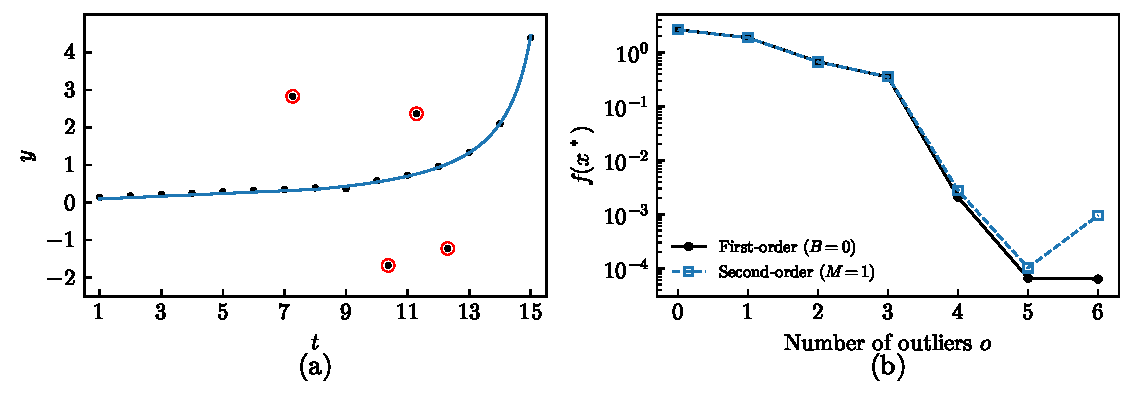
\includegraphics[width=\textwidth]{bard_panels.pdf}
\caption{Bard function with four added outliers, two above and two below the
model curve. (a) The fit returned at $o=4$ (solid line) follows the fifteen
clean observations (dots), while the four points identified as outliers
(circles) are discarded. (b) Best $f(x^*)$ over the $100$ starting points as a
function of the number $o$ of discarded observations (logarithmic vertical axis;
the two variants coincide): $f(x^*)$ decreases only moderately up to $o=3$ and
drops by more than two orders of magnitude at $o=4$, after which it stays at the
residual floor of the clean data, the onset of which identifies the four
outliers.}
\label{fig:bard}
\end{figure}

Unlike the polynomial instance, the counts now differ between the two methods,
and the difference has structure. The aggregate over all $o$ is dominated by
$o = 0$---the minimax over all $m = 19$ observations, outliers included---a hard
nonconvex problem where both methods are expensive (about $360$--$400$ mean
iterations) and the first-order method is in fact slightly cheaper. Once at
least the outliers are being discarded ($o \ge 1$), the regime for which the
method is intended, the second-order variant is more efficient in aggregate. The
comparison is not uniform row by row: the first-order method has the lower mean
iteration count at $o = 2$ and $o = 6$, the lower mean evaluation count at
$o = 2$, and the lower median iteration count at $o = 5$ and $o = 6$. The one
metric that favors the second-order variant at every $o \ge 1$ is the median
evaluation count.
Summing the per-$o$ means of Table~\ref{tab:bard} over $o = 1, \dots, 6$ gives
$232$ iterations and $296$ evaluations for the first-order method against $114$
and $160$ for the second-order variant; the corresponding sums of the per-$o$
medians are $43.5$ and $115$ against $38$ and $83$. The mean gap is large---the
first-order method uses about twice as many iterations and evaluations---but is
amplified by a heavy tail of slow first-order runs on the hardest instances (at
$o = 1$ the mean iteration count is $152$ for the first-order method against
$39$ for the second-order variant), which the curvature mitigates. The median,
robust to this tail, still favors the second-order variant, though far more
modestly. Either way, in aggregate over this regime the curvature lowers the
cost.

Curvature thus helps precisely where the first-order model is a poor local
approximation---a nonlinear model with outliers still present---while it neither
helps on the affine model of Section~\ref{subsec:poly} nor on the full-data
minimax at $o = 0$. This is consistent with the analysis of
Section~\ref{sec:complexity}, where the curvature affects only the constants of the
complexity bounds: the gain is a constant-factor one, realized here in the
outlier-rich regime, not a change in the order. One caveat tempers it: once the
outliers are removed ($o \ge 4$) both
methods reach the residual floor of the clean data, where the first-order
variant attains the lower $f(x^*)$ values, by a factor of about $15$ at
$o = 6$. A second caveat, the per-iteration cost of the curvature, is examined
next.

\subsection{Computational cost} \label{subsec:time}

Iteration and evaluation counts do not reflect the extra work the second-order
variant performs at every iteration: for each active component it assembles the
Hessian $\nabla^2 f_i(x^k)$, diagonalizes it, applies the shift \eqref{shift}
and rescales it, at a cost of one \texttt{DSYEV} call per index in
$I_\delta(x^k)$. Table~\ref{tab:time} therefore reports CPU times, measured with
the Fortran intrinsic \texttt{cpu\_time} around the call to the algorithm and
aggregated in the same way as the counts: for each $o$ we take the mean and the
median over the $100$ starting points, and the table sums those per-$o$ values
over the sweep.

\begin{table}[ht!]
\centering
\begin{tabular}{l cc cc cc}
\hline
 & \multicolumn{2}{c}{First-order ($B=0$)}
 & \multicolumn{2}{c}{Second-order ($M=1$)}
 & \multicolumn{2}{c}{ratio} \\
\cline{2-3}\cline{4-5}\cline{6-7}
 & mean & median & mean & median & mean & median \\
\hline
Polynomial, $o=0,\dots,12$
  & $115.7$ & $110.0$ & $158.9$ & $146.3$ & $1.37$ & $1.33$ \\
Bard, $o=0,\dots,6$
  & $62.2$  & $38.0$  & $51.4$  & $33.8$  & $0.83$ & $0.89$ \\
Bard, $o=1,\dots,6$
  & $35.1$  & $11.0$  & $29.2$  & $11.7$  & $0.83$ & $1.06$ \\
\hline
\end{tabular}
\caption{CPU time in milliseconds for the polynomial of
Section~\ref{subsec:poly} and the Bard function of Section~\ref{subsec:bard},
summed over the sweep in $o$. For each $o$
the mean and median over the $100$ starting points are taken, as in
Tables~\ref{tab:poly} and~\ref{tab:bard}, and those values are then summed. The
ratio columns give second-order over first-order, so that values below $1$
favour the second-order variant.}
\label{tab:time}
\end{table}

The two problems behave in opposite ways, and both are informative. On the
polynomial, where the counts were indistinguishable, the second-order variant
costs $37\%$ more time in the mean and $33\%$ more in the median: with nothing
to gain from the curvature, its assembly and diagonalization are pure overhead.
This quantifies the redundancy diagnosed in Section~\ref{subsec:poly}. On the
Bard problem the iteration savings more than pay for that overhead, and the
second-order variant is $17\%$ faster in the mean, both over the whole sweep and
over the regime $o \ge 1$. The medians again temper the conclusion: over the
whole sweep the second-order variant is $11\%$ faster, but restricted to
$o \ge 1$ it is $6\%$ \emph{slower}, because there the typical run of either
method terminates in a handful of iterations and the per-iteration overhead is
no longer amortized. The wall-clock advantage is therefore real but smaller than
the roughly twofold gap in mean iteration counts suggests, and it is confined to
the nonlinear problem.

We note that these times are of the order of tens of milliseconds and, being
averages over $100$ runs of a single sweep, carry some machine noise; the
ratios, not the absolute values, are the meaningful quantity.

\subsection{Sensitivity to $\delta$ and $\sigma_{\min}$} \label{subsec:sens}

The band half-width $\delta$ and the initial regularization $\sigma_{\min}$ are
chosen by trial and error, so it is natural to ask how much of the above depends
on that choice. We repeated the Bard experiment of Section~\ref{subsec:bard} for
every combination of $\delta \in \{10^{-1},10^{-2},10^{-3},10^{-4}\}$ and
$\sigma_{\min} \in \{10^{-1},10^{-2},10^{-3}\}$, with $\gamma$, $\alpha$,
$\epsilon$, $M$ and the $100$ starting points unchanged, and with both methods.
Table~\ref{tab:sens} collects the results.

\begin{table}[ht!]
\centering
\resizebox{\textwidth}{!}{%
\begin{tabular}{cc ccc cc cc}
\hline
 & & & &
 & \multicolumn{2}{c}{First-order ($B=0$)}
 & \multicolumn{2}{c}{Second-order ($M=1$)} \\
\cline{6-7}\cline{8-9}
$\delta$ & $\sigma_{\min}$ & $f(x^*)$ at $o=3$ & $f(x^*)$ at $o=4$ & drop
 & \#it & \#fcnt & \#it & \#fcnt \\
\hline
$10^{-1}$ & $10^{-1}$ & 3.511e-01 & 2.086e-03 & $168\times$ & 232 &  295 & 115 &  160 \\
$10^{-1}$ & $10^{-2}$ & 3.536e-01 & 1.591e-03 & $222\times$ &  54 &  174 &  46 &  130 \\
$10^{-1}$ & $10^{-3}$ & 3.493e-01 & 1.813e-03 & $193\times$ &  36 &  182 &  43 &  158 \\
$10^{-2}$ & $10^{-1}$ & 3.491e-01 & 1.783e-03 & $196\times$ & 258 &  413 & 170 &  285 \\
$10^{-2}$ & $10^{-2}$ & 3.489e-01 & 1.350e-03 & $258\times$ &  83 &  340 &  74 &  281 \\
$10^{-2}$ & $10^{-3}$ & 3.489e-01 & 1.386e-03 & $252\times$ &  65 &  387 &  76 &  340 \\
$10^{-3}$ & $10^{-1}$ & 3.487e-01 & 1.327e-03 & $263\times$ & 332 &  684 & 242 &  523 \\
$10^{-3}$ & $10^{-2}$ & 3.488e-01 & 1.338e-03 & $261\times$ & 148 &  694 & 121 &  551 \\
$10^{-3}$ & $10^{-3}$ & 3.488e-01 & 1.329e-03 & $262\times$ & 110 &  726 & 119 &  639 \\
$10^{-4}$ & $10^{-1}$ & 3.487e-01 & 1.304e-03 & $267\times$ & 427 & 1158 & 372 &  978 \\
$10^{-4}$ & $10^{-2}$ & 3.487e-01 & 1.291e-03 & $270\times$ & 219 & 1249 & 178 &  939 \\
$10^{-4}$ & $10^{-3}$ & 3.487e-01 & 1.293e-03 & $270\times$ & 171 & 1286 & 177 & 1168 \\
\hline
\end{tabular}%
}
\caption{Sensitivity of the Bard experiment to $\delta$ and $\sigma_{\min}$.
The values of $f(x^*)$ and the drop factor between $o=3$ and $o=4$ are those of
the first-order method; the second-order variant agrees with them to within the
multistart variability. The count columns give the mean \#it and \#fcnt over the
$100$ starting points, summed over $o=1,\dots,6$; small discrepancies with
Table~\ref{tab:bard} in the first row are due to rounding of the per-$o$ means
before summation. In all $24$ runs the $o=4$
solution identified exactly the four added outliers.}
\label{tab:sens}
\end{table}

Three things are stable across the table. The four outliers are identified
exactly in every one of the $24$ runs. The drop in $f(x^*)$ between $o=3$ and
$o=4$ is never smaller than two orders of magnitude, ranging from $168\times$ to
$270\times$. And the value of $f(x^*)$ at the plateau and at the floor varies
only in the third significant digit. The identification of the outliers, which
is what the method is used for, is therefore not an artefact of the particular
$\delta$ and $\sigma_{\min}$ reported in Section~\ref{subsec:bard}.

The counts, by contrast, do depend on the parameters, and in a way the analysis
anticipates. Decreasing $\delta$ raises the evaluation count steeply---at fixed
$\sigma_{\min}=10^{-1}$, from
about $300$ at $\delta=10^{-1}$ to about $1200$ at $\delta=10^{-4}$ for the
first-order method---which is consistent with the threshold
$9c_x^2/(2\delta)$ of Theorem~\ref{teo:suff-descent}: a narrower band forces a
larger $\sigma_{k,j}$, hence more rejected trial points per iteration. The
effect of $\sigma_{\min}$ is the opposite and milder, a smaller initial
regularization allowing longer early steps. Notably, the setting
$\delta=\sigma_{\min}=10^{-1}$ used in Section~\ref{subsec:bard}, inherited from
\cite{alvarezovo}, is the one with the largest iteration count in the table; we
keep it so that a single parameter set is used throughout the paper and the
comparison with the first-order method is made on its own terms.

The comparison between the two methods is likewise stable. The second-order
variant has the lower mean evaluation count in \emph{all twelve} parameter
combinations, and the lower mean iteration count in eight of the twelve; the
four exceptions all occur at the smallest value $\sigma_{\min}=10^{-3}$, and in
each of them the evaluation count still favours the second-order variant. The
advantage reported in Section~\ref{subsec:bard} is thus not an artefact of the
parameter choice either, though its size clearly is.

\section{Final remarks} \label{sec:final}

We have extended the first-order regularized method of \cite{alvarezovo} for
box-constrained order-value optimization by enriching its model with curvature,
each active component carrying its own positive semidefinite matrix of norm at
most $M$. The resulting method is well defined and, under the same
assumptions, attains worst-case iteration- and evaluation-complexity bounds of
the same order as its first-order counterpart (Theorem~\ref{teo:complexity}), of
which it is a strict generalization; the curvature enters only through the
constant $M$ in \eqref{cota-iter}, and not through the order of the bound. The
curvature is thus accommodated at no cost in the order of the theoretical
guarantees. Positive semidefiniteness and the bound $M$ are the only
requirements imposed on the matrices, so quasi-Newton updates such as BFGS or
SR1, Gauss--Newton matrices and shifted exact Hessians all fit directly into the
framework; individual positive semidefiniteness is used in
Theorem~\ref{teo:suff-descent} to make the model an upper approximation of each
active component, while only the convex combination $\bar{B}_{k,j}$ of
Corollary~\ref{cor:step} enters the complexity bound.

The numerical experiments delineate where the curvature helps and where it does
not. On the affine model the component Hessians are constant and the curvature
is exact but redundant, and the two variants are indistinguishable. On the
nonlinear model the picture depends on the regime: for the full-data minimax the
curvature does not help, but once outliers are being discarded---the regime for
which order-value optimization is intended---the second-order variant is the
more efficient of the two, reducing both the mean and the median iteration and
evaluation counts aggregated over that regime and, in particular, curbing a
heavy tail of slow first-order runs on the hardest instances. The sensitivity
study of Section~\ref{subsec:sens} shows that this is not an artefact of the
particular $\delta$ and $\sigma_{\min}$ chosen: over the twelve parameter
combinations tested, the second-order variant has the lower mean evaluation
count in all of them and the lower mean iteration count in eight, while the
identification of the four outliers is exact throughout. The advantage is a
constant-factor one, realized where the first-order model is a poor local
approximation, and is consistent with the complexity analysis, in which the
curvature enters only the constants and not the order of the bounds. It should
be read with two caveats. First, the per-iteration cost of assembling,
diagonalizing, shifting and rescaling one curvature matrix per active component
is not reflected in the evaluation count; measuring it directly
(Section~\ref{subsec:time}) shows that on the affine model, where the counts are
identical, the second-order variant costs $37\%$ more CPU time in the mean and
$33\%$ more in the median, while on the nonlinear model the iteration savings
outweigh the overhead and it is $17\%$ faster in the mean, though only
marginally so, or slightly slower, in the median. Second, the solution quality
is essentially the same for both variants, with the first-order method reaching
lower values once the outliers have been discarded, by a factor of about $15$ at
$o = 6$.

The reason the curvature does not change the order is structural. The Tikhonov
term $\sigma\|x - \bar x\|^2$ makes the model an upper approximation of $f$ once
$\sigma$ is of order $L$, which bounds the accepted step from below by a
multiple of $\epsilon$ at every iteration at which $C_{\delta,\epsilon}$ fails,
hence a per-iteration decrease of order $\epsilon^2$ and the $O(\epsilon^{-2})$
iteration bound. A natural way to
genuinely improve the order is to replace the quadratic regularization by a
cubic one, $\tfrac{\sigma}{3}\|x - \bar x\|^3$, in the spirit of the
cubic-regularization method of \cite{nesterov} and the high-order regularized
models of \cite{bgmst1, bgms}. With accurate second-order information---the true
or Gauss--Newton Hessian of each active component, used unmodified rather than
shifted and rescaled to meet an arbitrary bound $M$---and under the additional
assumption that the component Hessians are
Lipschitz continuous, the cubic model is an upper approximation with a step of
size $O(\epsilon^{1/2})$ and a per-iteration decrease of order $\epsilon^{3/2}$,
which would improve the iteration bound to $O(\epsilon^{-3/2})$. Realizing this
for the order-value function is not a direct transfer: the objective is
nonsmooth, the complexity carries the two parameters $\delta$ and $\epsilon$, and
the approximate optimality condition $C_{\delta,\epsilon}$ is stated in terms of
active gradients. Extending the analysis to a cubically regularized model,
tracking the interaction of the improved $\epsilon$-dependence with $\delta$, is
a promising direction in which the curvature would acquire a provable role, at
the price of a stronger smoothness assumption, accurate second-order information,
and a cubically regularized subproblem.

\section*{Declarations}

\medskip
\noindent
\textbf{Funding.} This work was funded by the Vice-Rectorate for Research, Outreach and Social Projection of the University of the Atlantic through the 2022 Internal Call for Proposals to Strengthen Research Groups with Tools for Creation, Innovation, and Research (award code CB734-CII2023).

\medskip
\noindent
\textbf{Conflicts of interest.} The authors have no relevant financial or non-financial interests to disclose.

\medskip
\noindent
\textbf{Data and code availability.} The polynomial data set of Section~\ref{subsec:poly} is the one of \cite{dunder1}. The data of Section~\ref{subsec:bard} consist of the 15 observations of the Bard function listed in \cite{mgh} together with four outliers generated with a fixed random seed, as described there. The Fortran 90 implementation of Algorithm~\ref{alg:main}, both data sets, and the scripts that reproduce every table and figure of Section~\ref{sec:numerical} are openly available at \url{https://github.com/gdquintero/ovoqnewton}.

\medskip
\noindent
\textbf{Authors' contributions.} All authors contributed to the conception and design of the study, to the analysis, and to the writing of the manuscript. All authors read and approved the final manuscript.

\medskip
\noindent
\textbf{Acknowledgements.} The authors thank the University of the Atlantic and its Vice-Rectorate for Research, Outreach and Social Projection for granting access to the Centro de Modelación Matemática.

\clearpage

\begin{thebibliography}{99}

\bibitem{dunder1} R. Andreani, C. Dunder and J. M. Mart\'{\i}nez, Order-Value Optimization: Formulation and solution by means of a primal Cauchy method, \textit{Mathematical Methods of Operations Research} 58, pp. 387--399, 2003.

\bibitem{dunder2} R. Andreani, C. Dunder and J. M. Mart\'{\i}nez, Nonlinear-programming reformulation of the order-value optimization problem, \textit{Mathematical Methods of Operations Research} 61, pp. 365--384, 2005.

\bibitem{yano1} R. Andreani, J. M. Mart\'{\i}nez, M. Salvatierra, and F. S. Yano, Quasi-Newton methods for Order-Value Optimization and Value-at-Risk calculations, \textit{Pacific Journal of Optimization} 2, pp. 11--33, 2006.

\bibitem{yano2} R. Andreani, J. M. Mart\'{\i}nez, L. Mart\'{\i}nez, and F. S. Yano, Low order-value optimization and applications, \textit{Journal of Global Optimization} 43, pp. 1--22, 2009.

\bibitem{salva} R. Andreani, J. M. Mart\'{\i}nez, M. Salvatierra, and F. S. Yano, Global order-value optimization by means of a multistart harmonic oscillator tunneling strategy, in \textit{Global Optimization: From Theory to Implementation}, L. Liberti and N. Maculan (eds.), Springer, Boston, MA, 2006, pp. 379--404.

\bibitem{bgms} E. G. Birgin, J. L. Gardenghi, J. M. Mart\'{\i}nez, and S. A. Santos, On the use of third-order models with fourth-order regularization for unconstrained optimization, \textit{Optimization Letters} 14, pp. 815--838, 2020.

\bibitem{bgmst2} E. G. Birgin, J. L. Gardenghi, J. M. Mart\'{\i}nez, S. A. Santos, and Ph. L. Toint, Evaluation complexity for nonlinear constrained optimization using unscaled KKT conditions and high-order models, \textit{SIAM Journal on Optimization} 26, pp. 951--967, 2016.

\bibitem{bgmst1} E. G. Birgin, J. L. Gardenghi, J. M. Mart\'{\i}nez, S. A. Santos, and Ph. L. Toint, Worst-case evaluation complexity for unconstrained nonlinear optimization using high-order regularized models, \textit{Mathematical Programming} 163, pp. 359--368, 2017.

\bibitem{bmbook} E. G. Birgin and J. M. Mart\'{\i}nez, \textit{Practical Augmented Lagrangian Methods for Constrained Optimization}, Society for Industrial and Applied Mathematics, Philadelphia, 2014.

\bibitem{bmcomper} E. G. Birgin and J. M. Mart\'{\i}nez, Complexity and performance of an Augmented Lagrangian algorithm, \textit{Optimization Methods and Software} 35, pp. 885--920, 2020.

\bibitem{cogtbook} C. Cartis, N. I. M. Gould, and Ph. L. Toint, \textit{Evaluation Complexity of Algorithms for Nonconvex Optimization: Theory, Computation, and Perspectives}, SIAM, Philadelphia, PA, 2022.

\bibitem{gauvin} J. Gauvin, A necessary and sufficient regularity condition to have bounded multipliers in nonconvex programming, \textit{Mathematical Programming} 12, pp. 136--138, 1977.

\bibitem{jorion} P. Jorion, \textit{Value at {R}isk: {T}he new benchmark for managing financial risk}, 3rd. ed., McGraw-Hill, 2009.

\bibitem{mtop} J. M. Mart\'{\i}nez, Generalized Order-Value Optimization, \textit{TOP} 20, pp. 75--98, 2012.

\bibitem{mgh} J. J. Mor\'e, B. S. Garbow, and K. E. Hillstrom, Testing unconstrained optimization software, \textit{ACM Transactions on Mathematical Software} 7, pp. 17--41, 1981.

\bibitem{nesterov} Y. Nesterov and B. T. Polyak, Cubic regularization of Newton method and its global performance, \textit{Mathematical Programming} 108, 177--205, 2006.

\bibitem{jiang} Z. Jiang, Q. Hu, and X. Zheng, Optimality condition and complexity of order-value optimization problems and low order-value optimization problems, \textit{Journal of Global Optimization} 69, pp. 511--523, 2017.

\bibitem{alvarezovo} G. Q. Álvarez and E. G. Birgin, A first-order regularized approach to the order-value optimization problem, \textit{Optimization Methods and Software} 40, pp. 650--674, 2025.
    
\end{thebibliography}

\end{document}